\section{Introduction}
\frame{\tableofcontents[currentsection]}


\begin{frame}
    \frametitle{Problem Statement (1)}
    \onslide<1->{
        Finite sample set $\fSet$, 
        cost function $\cost \colon \binom{\fSet}{3} \to \real$.\\
        Instance of the \textbf{Cubic Clique Partition Problem}:\\
        \[
        \min\limits_{\labels \colon \binom{\fSet}{2} \to \bSet}
        \sum\limits_{\{a,b,c\} \in \binom{\fSet}{3}}
        \cost_{\{a,b,c\}}\labels_{\{a,b\}}\labels_{\{b,c\}}\labels_{\{a,c\}} 
        \]
        subject to 
        $\labels_{\{a,b\}} + \labels_{\{b,c\}} - 1 \leq \labels_{\{a,c\}}$
        for all distinct $a,b,c \in \fSet$.    
    }
    \vspace{25px}
    \onslide<2->{
        Find a \textbf{partially optimal solution}, i.e.
        fix some labels $\labels_{\{a,b\}}$
        for distinct $a,b \in \fSet$
        \[
        \begin{cases}
            \labels_{\{a,b\}}=1 & \text{join } a,b\\
            \labels_{\{a,b\}}=0 & \text{cut } a,b\\
            \labels_{\{a,b\}}=\text{?} & \text{unknown}
        \end{cases}
        \]
        in such way that there still exists
        an optimal solution. 
    }
\end{frame}

\begin{frame}
    \frametitle{Problem Statement (2)}
    \textbf{Subspace Instances} of the Cubic Clique Partition Problem
    \vspace{5px}
    \onslide<1->{
        Samples $\fSet$: points $\fSet \subset \real^3$\\
    }
    \onslide<2->{
        Point generation: 3 distinct planes containing the origin, noise $\noise$\\
    }
    \onslide<3->{
        Optimal clustering $\labels^*$: original planes\\
    }
    \onslide<4->{
        Cost function $\cost$? (no concrete plane information given)
    }
    \begin{figure}[h]
    \centering
        \onslide<1->{
            \begin{subfigure}{0.4\textwidth}
                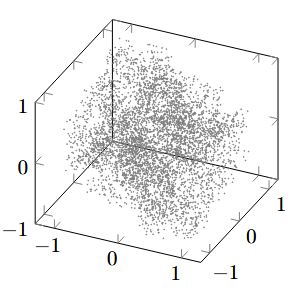
\includegraphics[width=\textwidth]{gray-points}
                \caption{Samples $\fSet$}
            \end{subfigure}
        }
        \hfill
        \onslide<2->{
            \begin{subfigure}[b]{0.4\textwidth}
                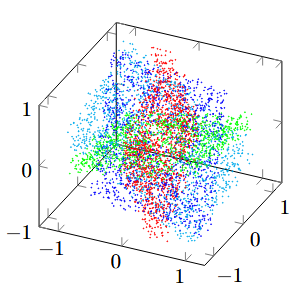
\includegraphics[width=\textwidth]{colored-points}
                \caption{Optimal clustering $\labels^*$}
            \end{subfigure}
        }
        \hspace{0.1\textwidth}
    \end{figure}
\end{frame}


\begin{frame}
    \frametitle{Research Goals and Contributions}
    \begin{tabularx}{\textwidth}{p{0.5\textwidth}|X}
        \textbf{Task} & \textbf{Solution}\\
        \hline 
        \onslide<1->{
        \vspace{-7px}
        read
        `Partial Optimality in Cubic Correlation Clustering'
        \cite{TODO};
        implement the algorithm for establishing partial optimality
        to the cubic clique partition problem;
        } &
        \onslide<2->{
        \vspace{-7px}
        my own implementation in C++ of the suggested
        algorithm with some adjustments
        \\
        \hline
        }
        \onslide<3->{
        \vspace{-7px}
        construct subspace instances
        of increasing difficulty
        by generating the sample points
        and by defining a
        \textbf{suitable cost function}
        for the point triples
        } &
        \onslide<4->{
        \vspace{-7px}
        point generation using the linear algebra methods;
        experimentally determined geometric
        cost function 
        with a significant noise tolerance;
        \\
        \hline
        }
        \onslide<5->{
        \vspace{-7px}
        apply the algorithm to the constructed subspace instances,
        assess partial optimality, accuracy with respect to
        truth, and computation time
        } &
        \onslide<6->{
        \vspace{-7px}
        systematic empirical assessment
        of the algorithm application to the problem subspace instances 
        with my cost function proving its quality
        }
    \end{tabularx}
\end{frame}